\documentclass[aspectratio=169]{beamer}
\usetheme{Madrid}
\usepackage{multicol}
\usepackage{tikz}
\usetikzlibrary{shapes.geometric, arrows}
\usecolortheme{default}

\title{SELF-DISCOVER: LLMs Self-Compose Reasoning Structures}
\subtitle{Authors: Pei Zhou et al., 2023 (University of Southern California, Google DeepMind)}
\author{Presenter: T Jones}
\institute{AI Journal Club}
\date{\today}

\begin{document}

\begin{frame}
\titlepage
\end{frame}

\begin{frame}

\begin{figure}
    \centering
    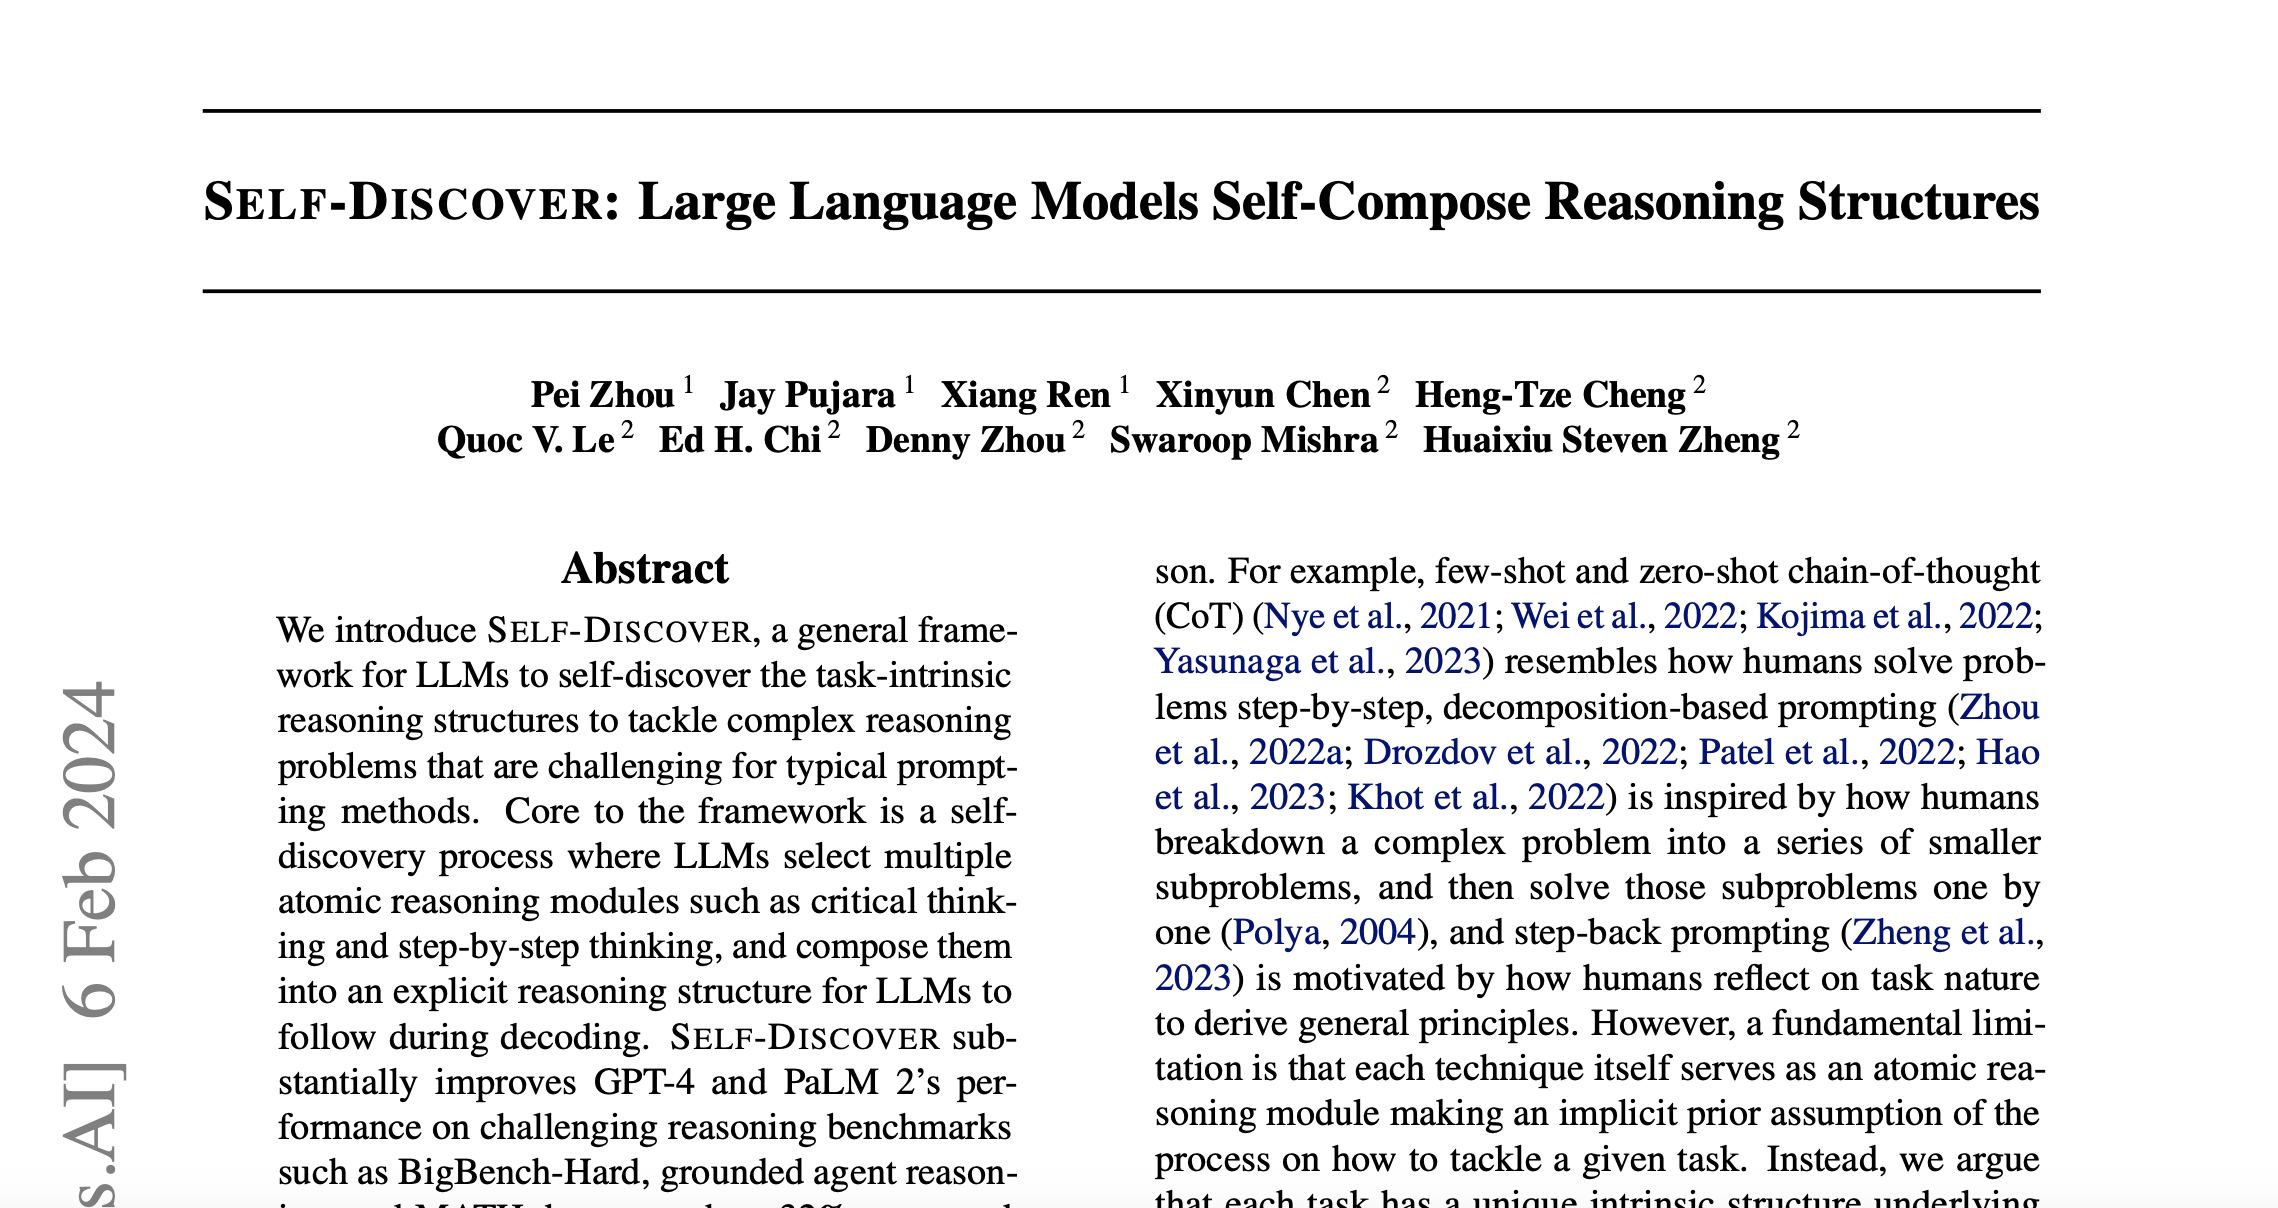
\includegraphics[width=1\linewidth]{paper.png}
    
    
\end{figure}
    
\end{frame}

\begin{frame}{How do {\it you} think?}
  \begin{columns}
    \begin{column}{0.7\textwidth}
        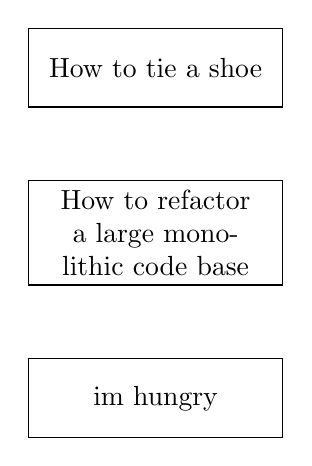
\begin{tikzpicture}[node distance=2cm]
        
            \node (problem1) [rectangle, draw, text width=3cm, text centered, minimum height=1cm] {How to tie a shoe};
            \node (problem2) [rectangle, draw, text width=3cm, text centered, minimum height=1cm, below of=problem1, yshift=-0.1cm] {How to refactor a large monolithic code base};
            \node (problem3) [rectangle, draw, text width=3cm, text centered, minimum height=1cm, below of=problem2, yshift=-0.1cm] {im hungry};
            
        
        \end{tikzpicture}
    \end{column}
    \begin{column}{0.3\textwidth}

    Do you think about these things with the exact same mental process?
      
    \end{column}
  \end{columns}
\end{frame}


\begin{frame}{How do {\it you} think?}
  \begin{columns}
    \begin{column}{0.7\textwidth}
        \begin{tikzpicture}[node distance=2cm]
        
            \node (problem1) [rectangle, draw, text width=3cm, text centered, minimum height=1cm] {How to tie a shoe};
            \node (problem2) [rectangle, draw, text width=3cm, text centered, minimum height=1cm, below of=problem1, yshift=-0.1cm] {How to refactor a large monolithic code base};
            \node (problem3) [rectangle, draw, text width=3cm, text centered, minimum height=1cm, below of=problem2, yshift=-0.1cm] {im hungry};
            
            \node (cot) [rectangle, draw, text width=3cm, text centered, minimum height=1cm, right of=problem1, xshift=3cm] {Chain of Thought/Habit};
            \node (ltm) [rectangle, draw, text width=3cm, text centered, minimum height=1cm, right of=problem2, xshift=3cm] {Least to Most/Decomp};
            \node (food) [rectangle, draw, text width=3cm, text centered, minimum height=1cm, right of=problem3, xshift=3cm] {hunter/gatherer instinct};

            \draw [arrow] (problem1) -- (cot);
            \draw [arrow] (problem2) -- (ltm);
            \draw [arrow] (problem3) -- (food);
        
        \end{tikzpicture}
    \end{column}
    \begin{column}{0.3\textwidth}
       \pause
      Your human brain does {\bf not} use one single mode of thinking to solve every problem. Rather, it picks the right problem-solving mode to fit the problem.
    \end{column}
  \end{columns}
\end{frame}

\begin{frame}{How do {\it LLMs} ``think"?}

\begin{itemize}
    \item Whether or not they actually ``think" $\longrightarrow$ philosophers \pause
    \item Practically, they sometimes {\it appear} to ``think". That is, they exhibit responses to queries that if coming from a human mind we would associate with thinking. \pause
    \item Let's put ``think" in quotes to avoid the philosophers. \pause
    \item The mechanics of LLM "thinking" is under active investigation, but prompting can alter the outcome of this "thinking" for better or worse. \pause
    \item Can we empower LLMs to pick their own prompts for ``thinking" about a problem?
\end{itemize}

\end{frame}

\begin{frame}{Motivation (1)}
\begin{itemize}
    \item LLMs have achieved remarkable performance in language generation and instruction-following tasks
    \pause
    \item However, complex multi-step reasoning remains a challenge
    \pause
    \begin{itemize}
    \item Struggles in tasks requiring logical deduction, causal reasoning, mathematical problem-solving
    \pause
    \end{itemize}
    \item Existing prompting techniques make strong assumptions about the reasoning process
    \pause
    \begin{itemize}
    \item Direct Answer (assumes simple Q\&A) \pause
    \item Chain-of-Thought (CoT) assumes step-by-step reasoning \pause
    \item Least-to-Most assumes problem decomposition \pause
    \end{itemize}
\end{itemize}
\begin{figure}
    \centering
    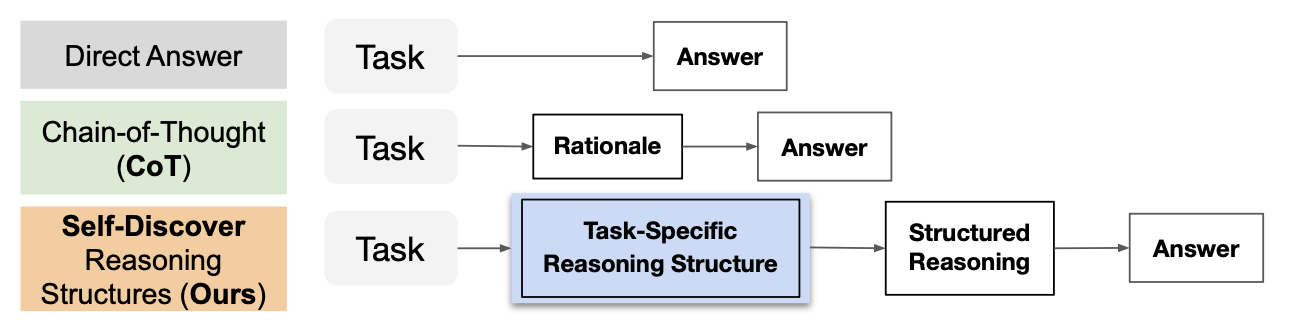
\includegraphics[width=0.7\linewidth]{prompt_types.png} 
\end{figure}
\end{frame}

\begin{frame}{Motivation (2)}
\begin{itemize}
    \item Key Insight: Each task has an intrinsic reasoning structure for efficient problem-solving \pause
    \begin{itemize}
        \item For example, a logical deduction $\longrightarrow$ sequence of premise-conclusion steps \pause
        \item A causal reasoning $\longrightarrow$ identifying cause-effect relationships and counterfactuals \pause
\end{itemize}
\end{itemize}
\end{frame}

\begin{frame}{Motivation (3)}
\begin{itemize}
    \item Uncovering the intrinsic reasoning structure can guide the model to solve the task more effectively \pause
    \begin{itemize}
    \item It provides a blueprint for the model to follow during problem-solving \pause
    \item It can reduce the search space of possible solutions \pause
    \item It enhances the interpretability of the model's problem-solving process \pause
    \end{itemize}
\end{itemize}
\end{frame}

\begin{frame}{Results}
\begin{figure}
    \centering
    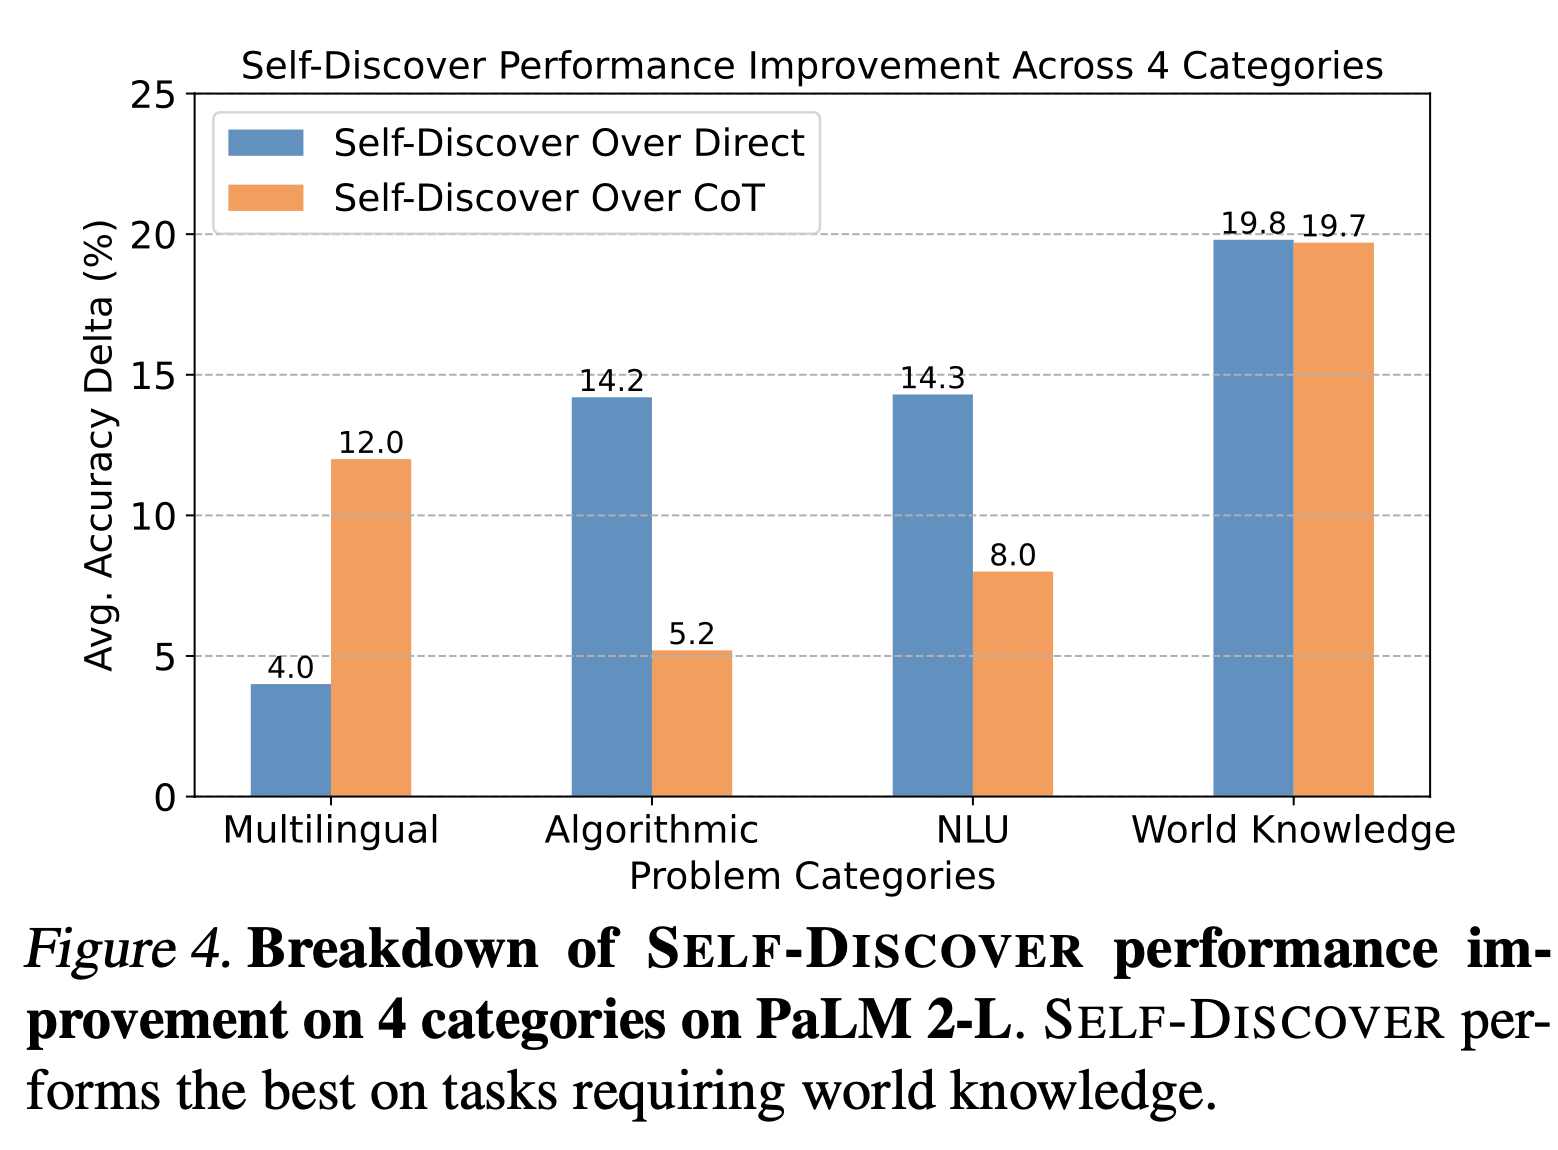
\includegraphics[width=0.65\linewidth]{results1.png}
\end{figure}
\end{frame}

\begin{frame}{Key Idea of SELF-DISCOVER}
\begin{itemize}
\item SELF-DISCOVER enables LLMs to uncover task-specific reasoning structures \pause
\begin{itemize}
\item Allows the model to adapt its reasoning to the intrinsic structure of the task \pause
\end{itemize}
\item The process begins by selecting from a set of atomic reasoning modules \pause
\begin{itemize}
\item Modules represent fundamental reasoning skills (e.g. critical thinking, problem decomposition) \pause
\item Modules are inspired cognitive science and LLM problem-solving literature (Google DeepMind's PROMPTBREEDER set), Modules are described in natural language \pause
\end{itemize}
\item SELF-DISCOVER composes the selected modules into a coherent reasoning structure \pause
\begin{itemize}
\item Composed structure reflects the LLM's intrinsic reasoning flow of the task  \pause
\item Performed in a few-shot setting, without requiring task-specific training data \pause
\end{itemize}
\item During inference, the model follows the self-discovered structure step-by-step \pause
\begin{itemize}
\item Each step corresponds to a selected reasoning module \pause
\item The model applies the skills associated with each module to progressively solve the task
\end{itemize}
\end{itemize}
% \begin{center}
% \includegraphics<13>[width=0.8\textwidth]{images/self_discover_overview.png}
% \end{center}
\end{frame}

\begin{frame}{Overview}
    \begin{figure}
    \centering
    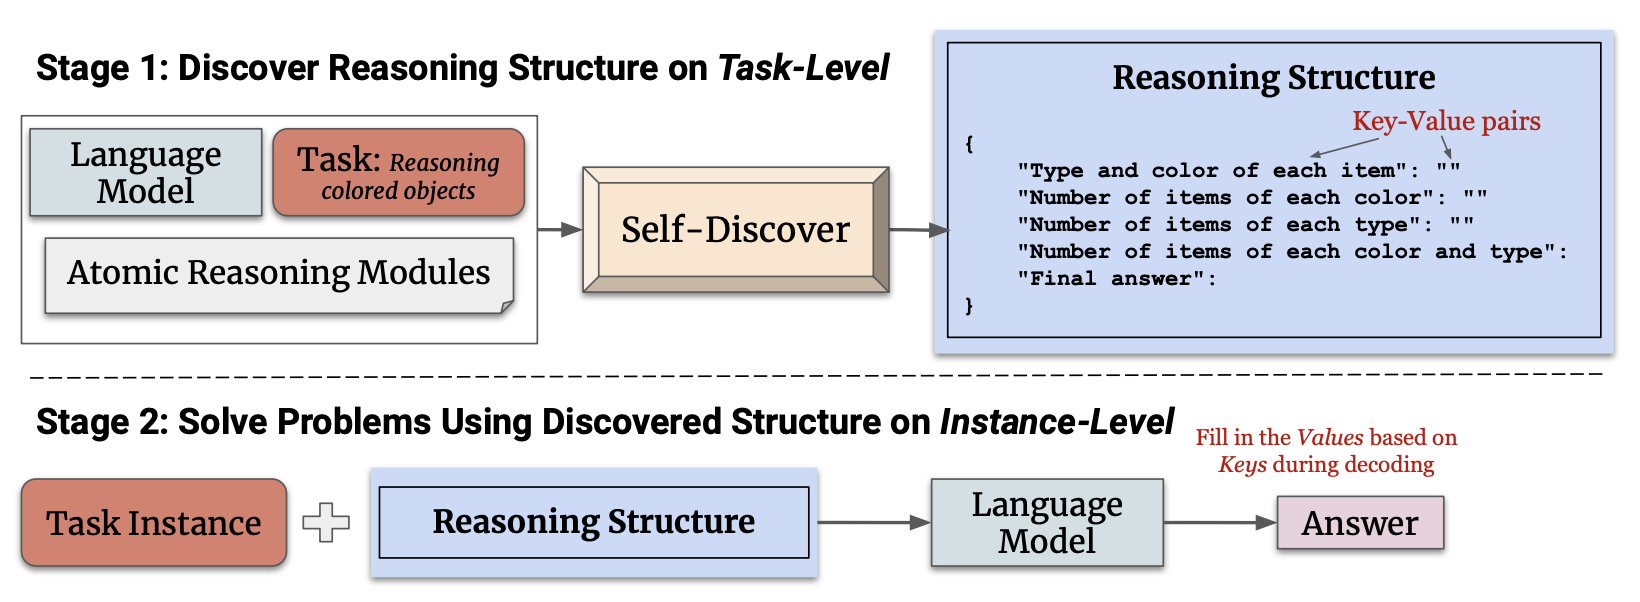
\includegraphics[width=1\linewidth]{image002.png}
\end{figure}
\end{frame}

\begin{frame}{Three stages}
Three key actions:
\begin{enumerate}
\item SELECT relevant reasoning modules
\item ADAPT module descriptions to task
\item IMPLEMENT into operational key-value structure
\end{enumerate}
\pause
\begin{columns}
\begin{column}{0.3\textwidth}
\begin{figure}
    \centering
    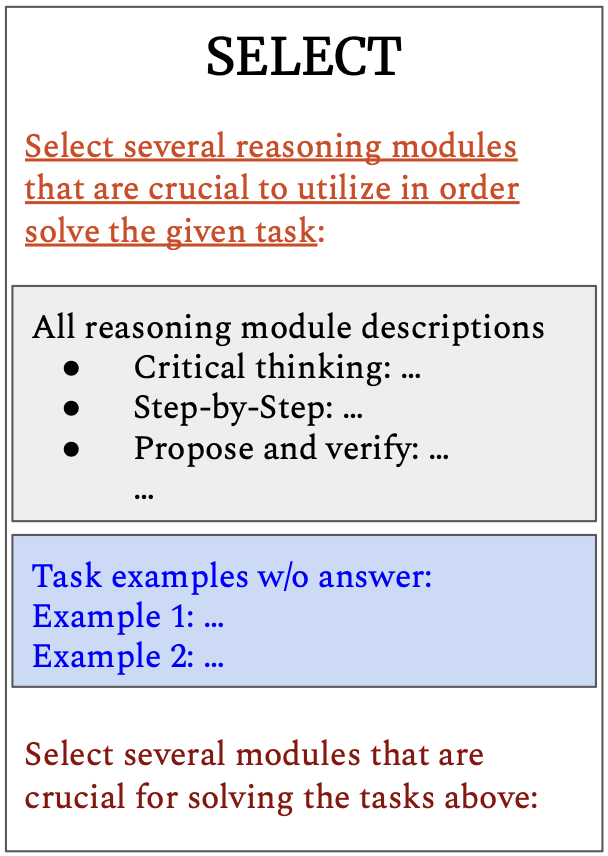
\includegraphics[width=0.8\linewidth]{select.png}
\end{figure}
\end{column}
\pause
\begin{column}{0.3\textwidth}
\begin{figure}
    \centering
    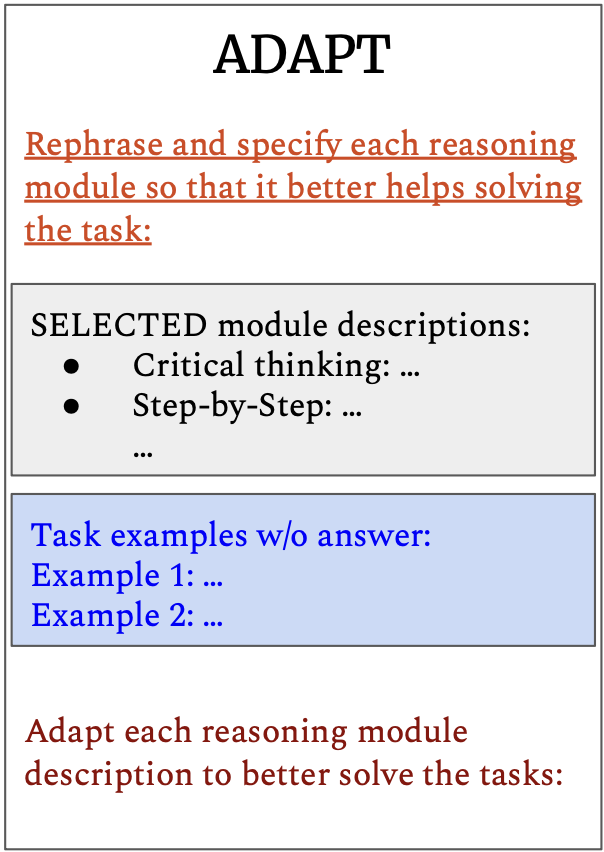
\includegraphics[width=0.8\linewidth]{adapt.png}
\end{figure}
\end{column}
\pause
\begin{column}{0.3\textwidth}
\begin{figure}
    \centering
    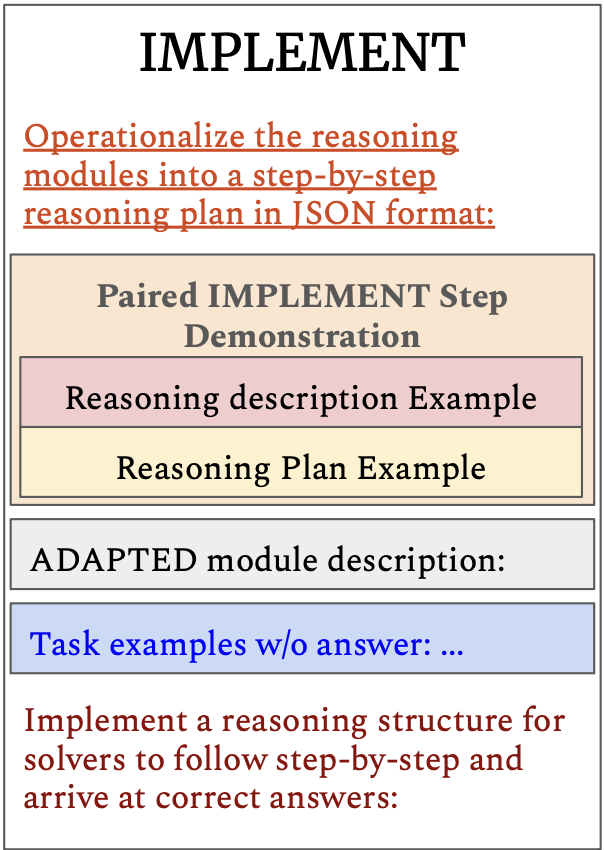
\includegraphics[width=0.8\linewidth]{implement.png}
\end{figure}
\end{column}
\end{columns}
\end{frame}

\begin{frame}{Reasoning Modules (0)}

\begin{figure}
    \centering
    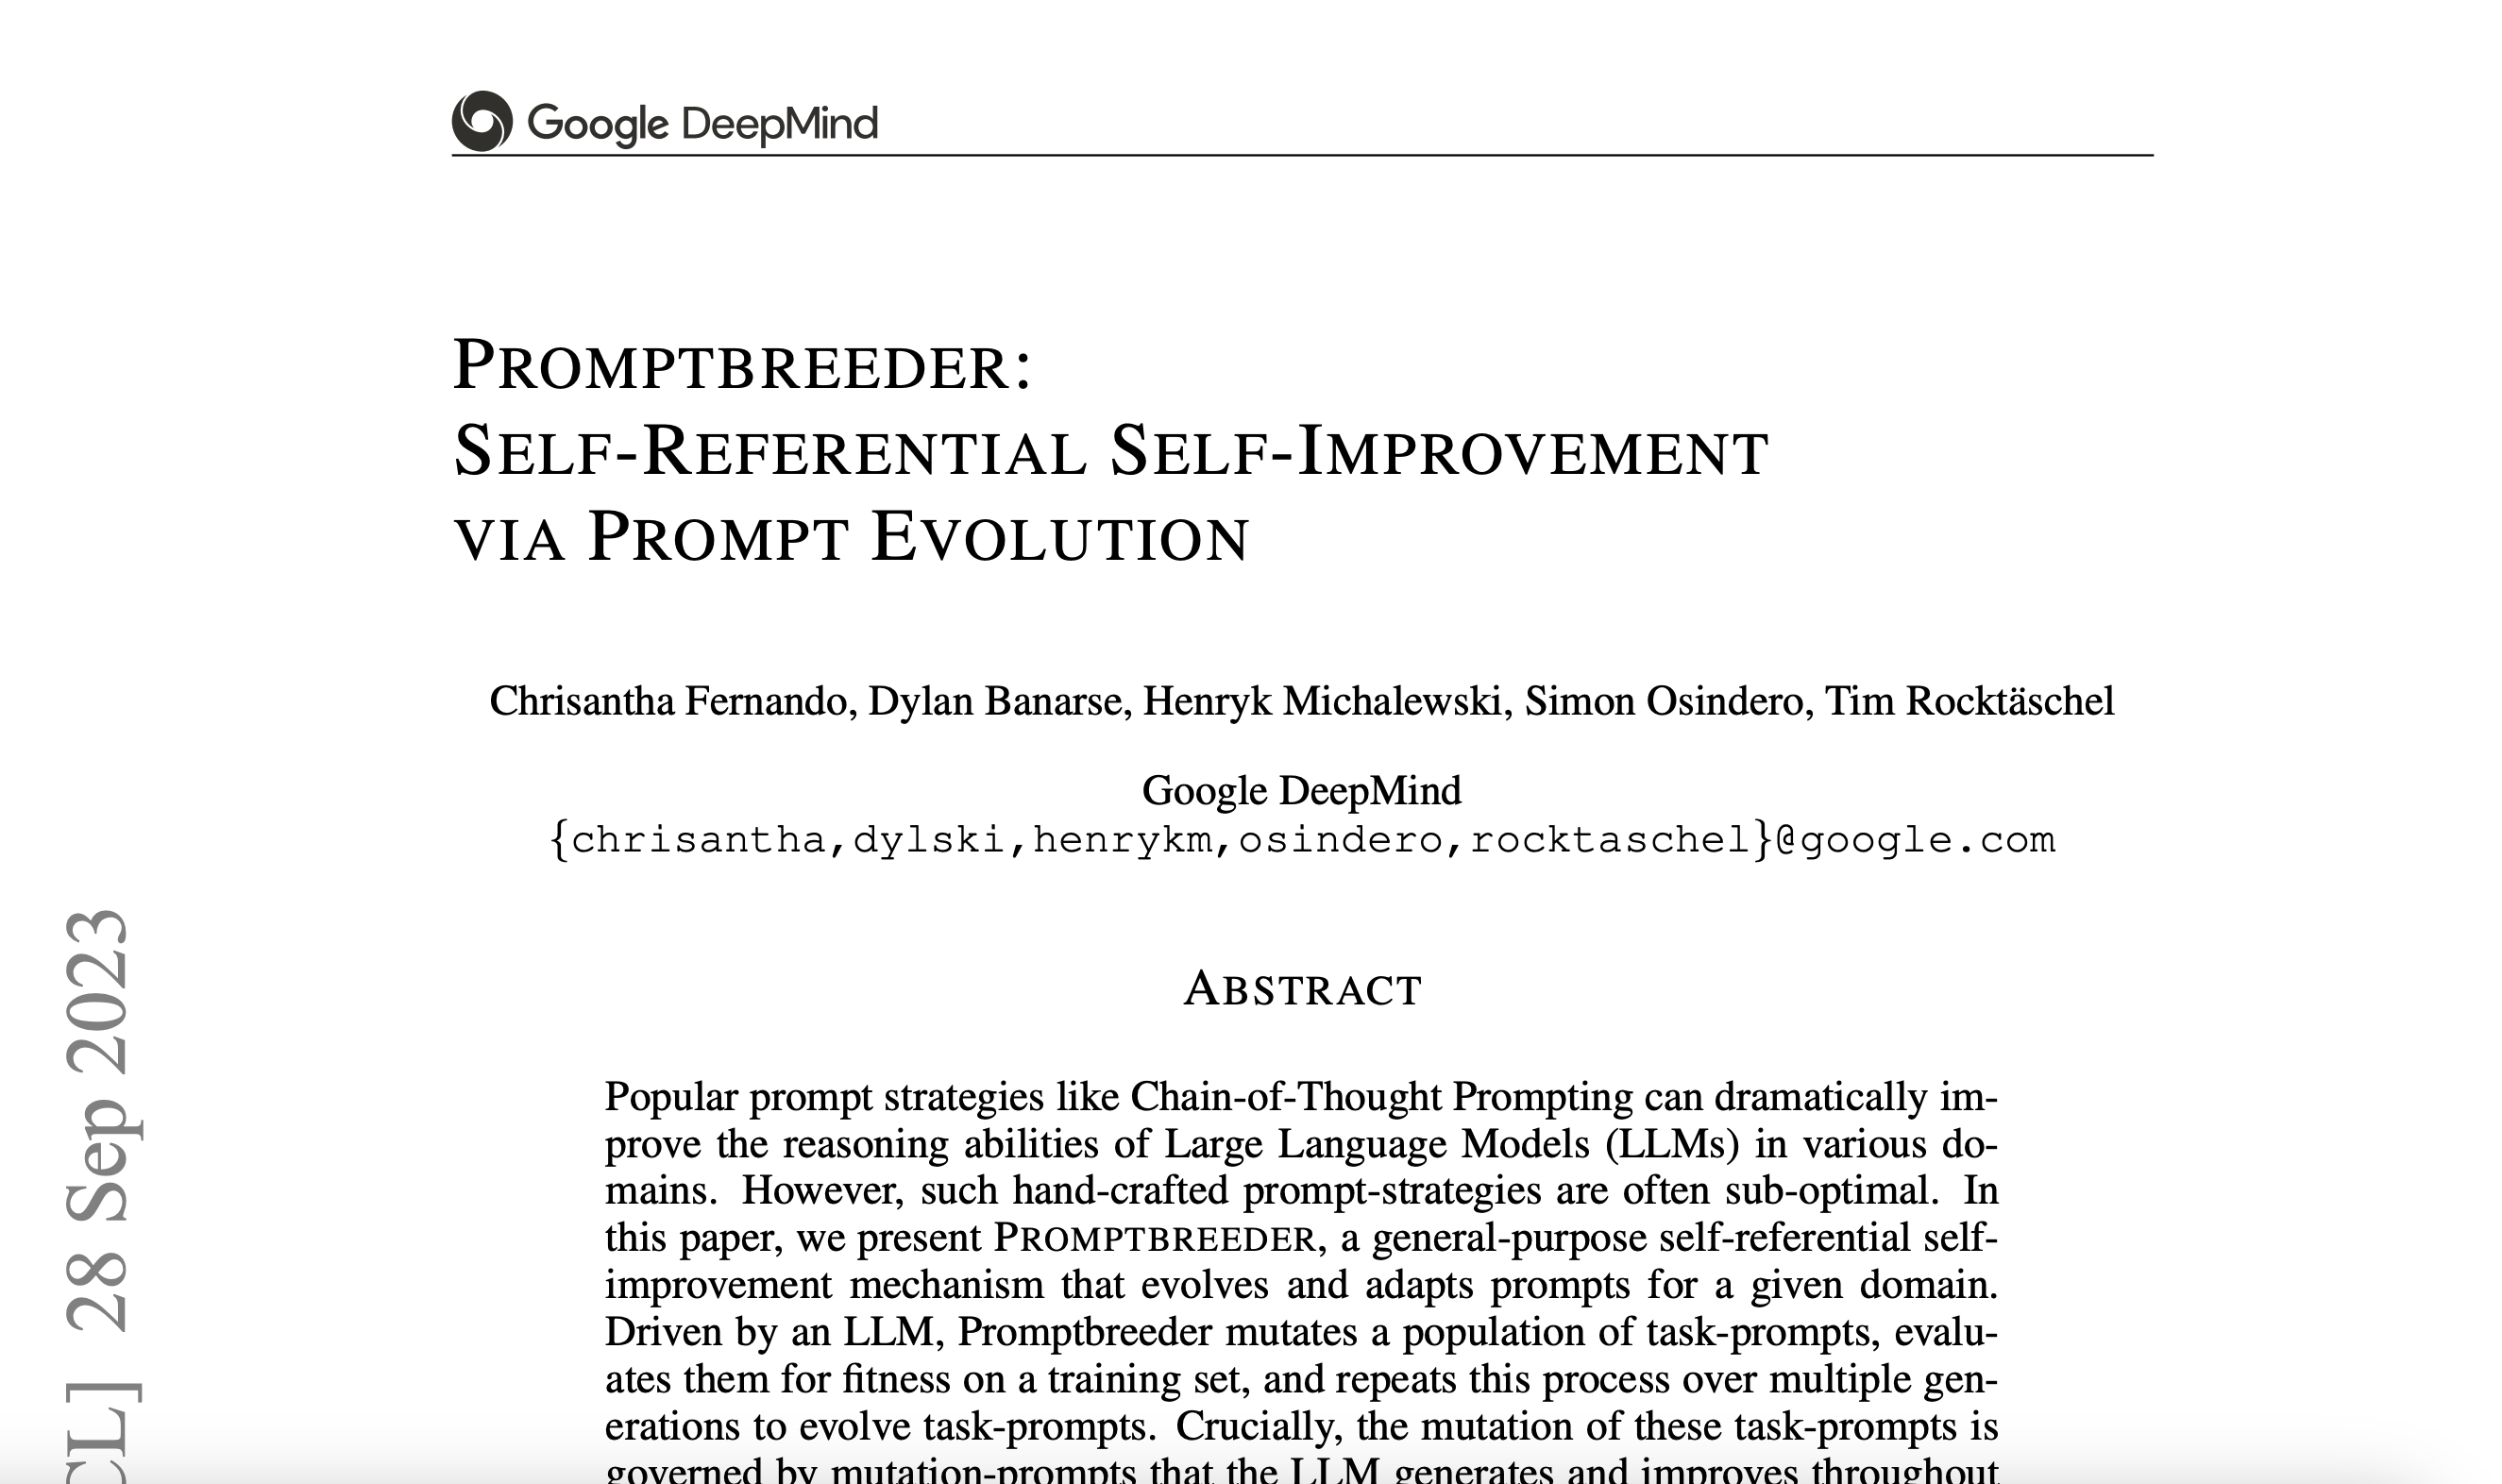
\includegraphics[width=0.75\linewidth]{prompt_paper.png}
    
\end{figure}

\end{frame}


\begin{frame}{Reasoning Modules (1)}

\begin{figure}
    \centering
    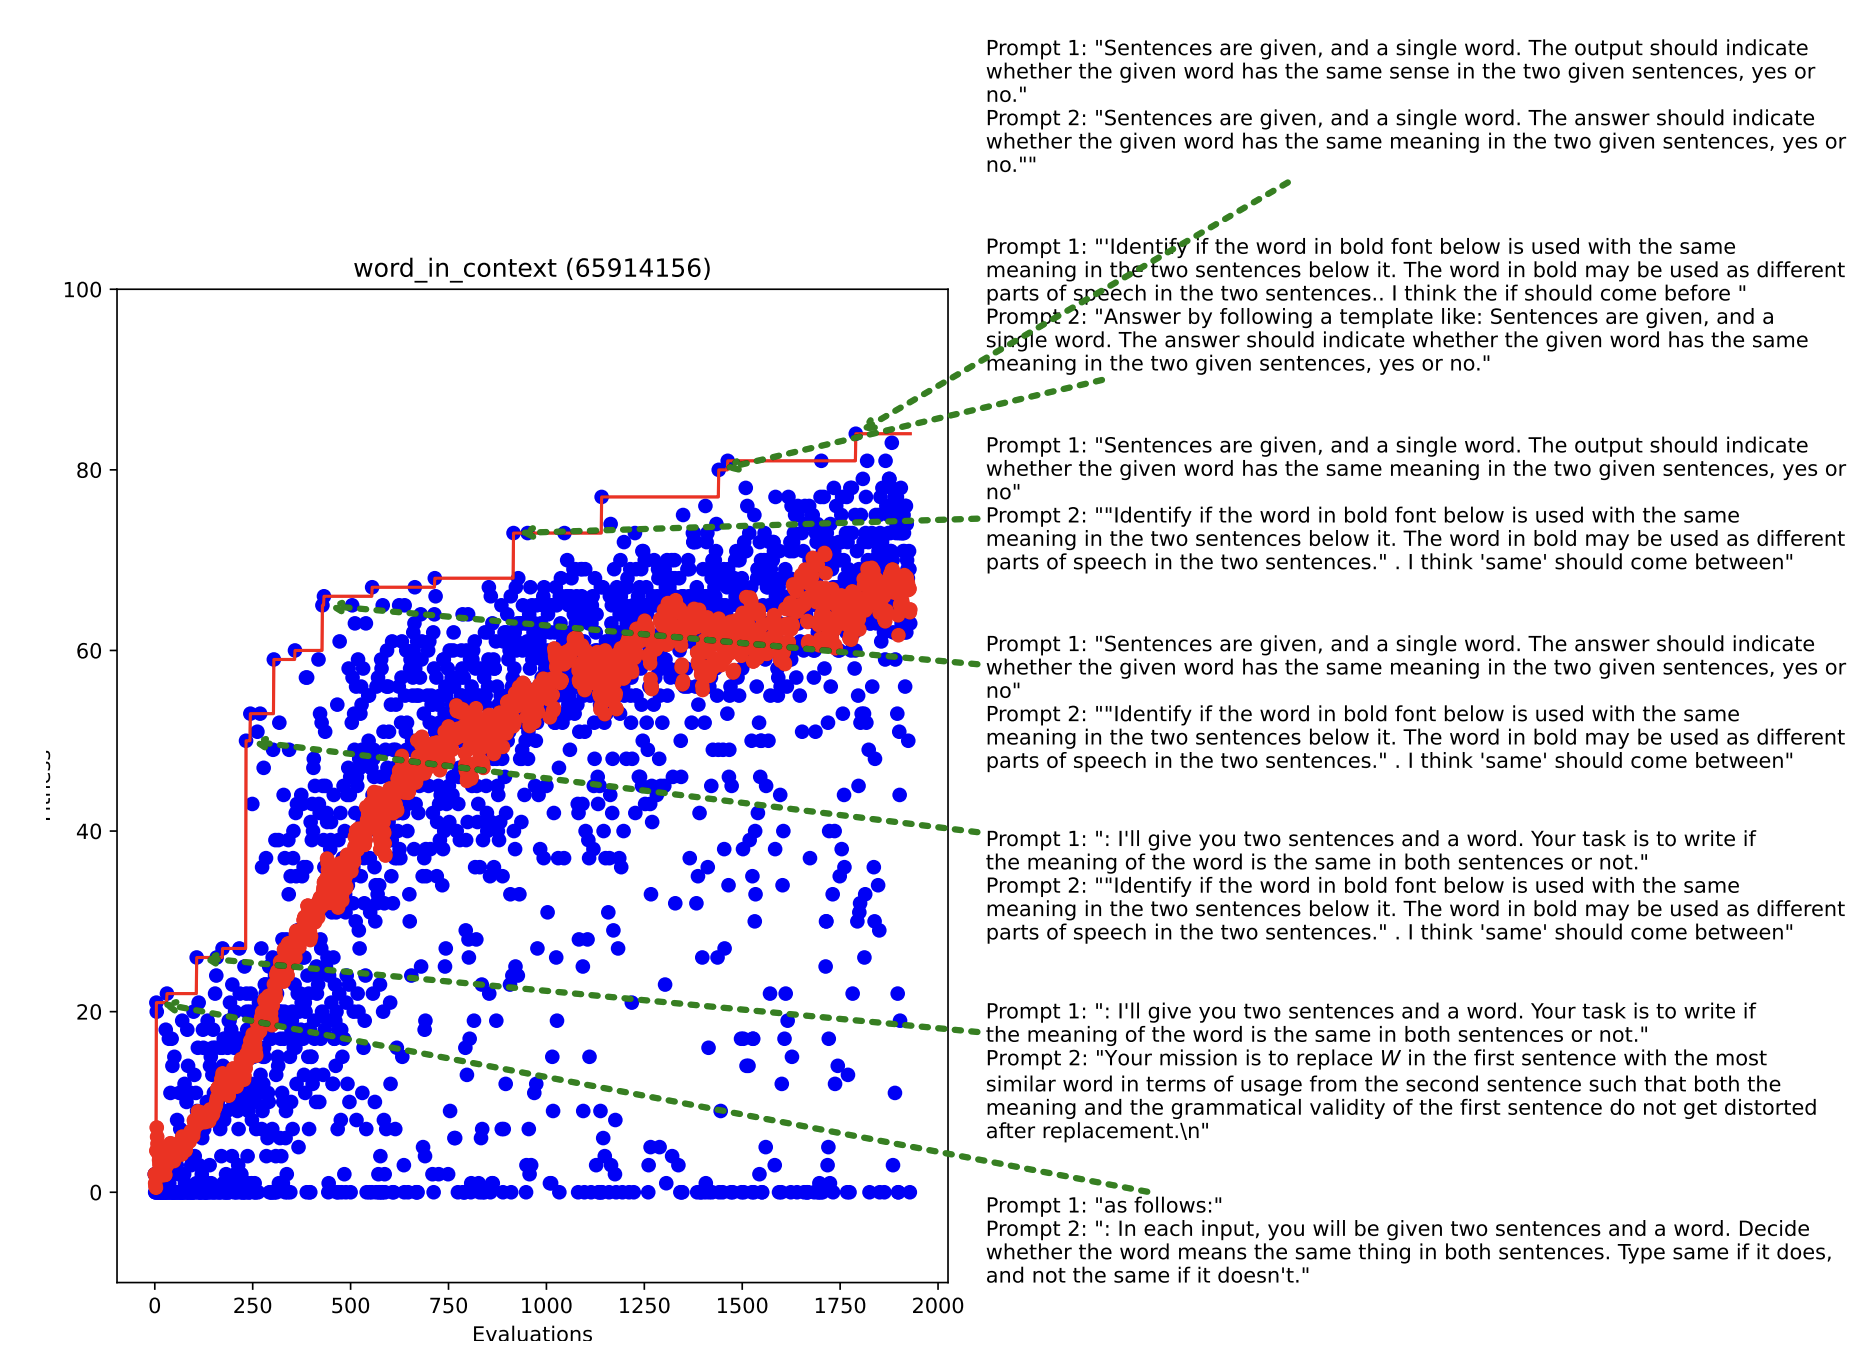
\includegraphics[width=0.65\linewidth]{prompt_b_example.png}
    
    
\end{figure}

\end{frame}



\begin{frame}{Reasoning Modules (2)}

\begin{figure}
    \centering
    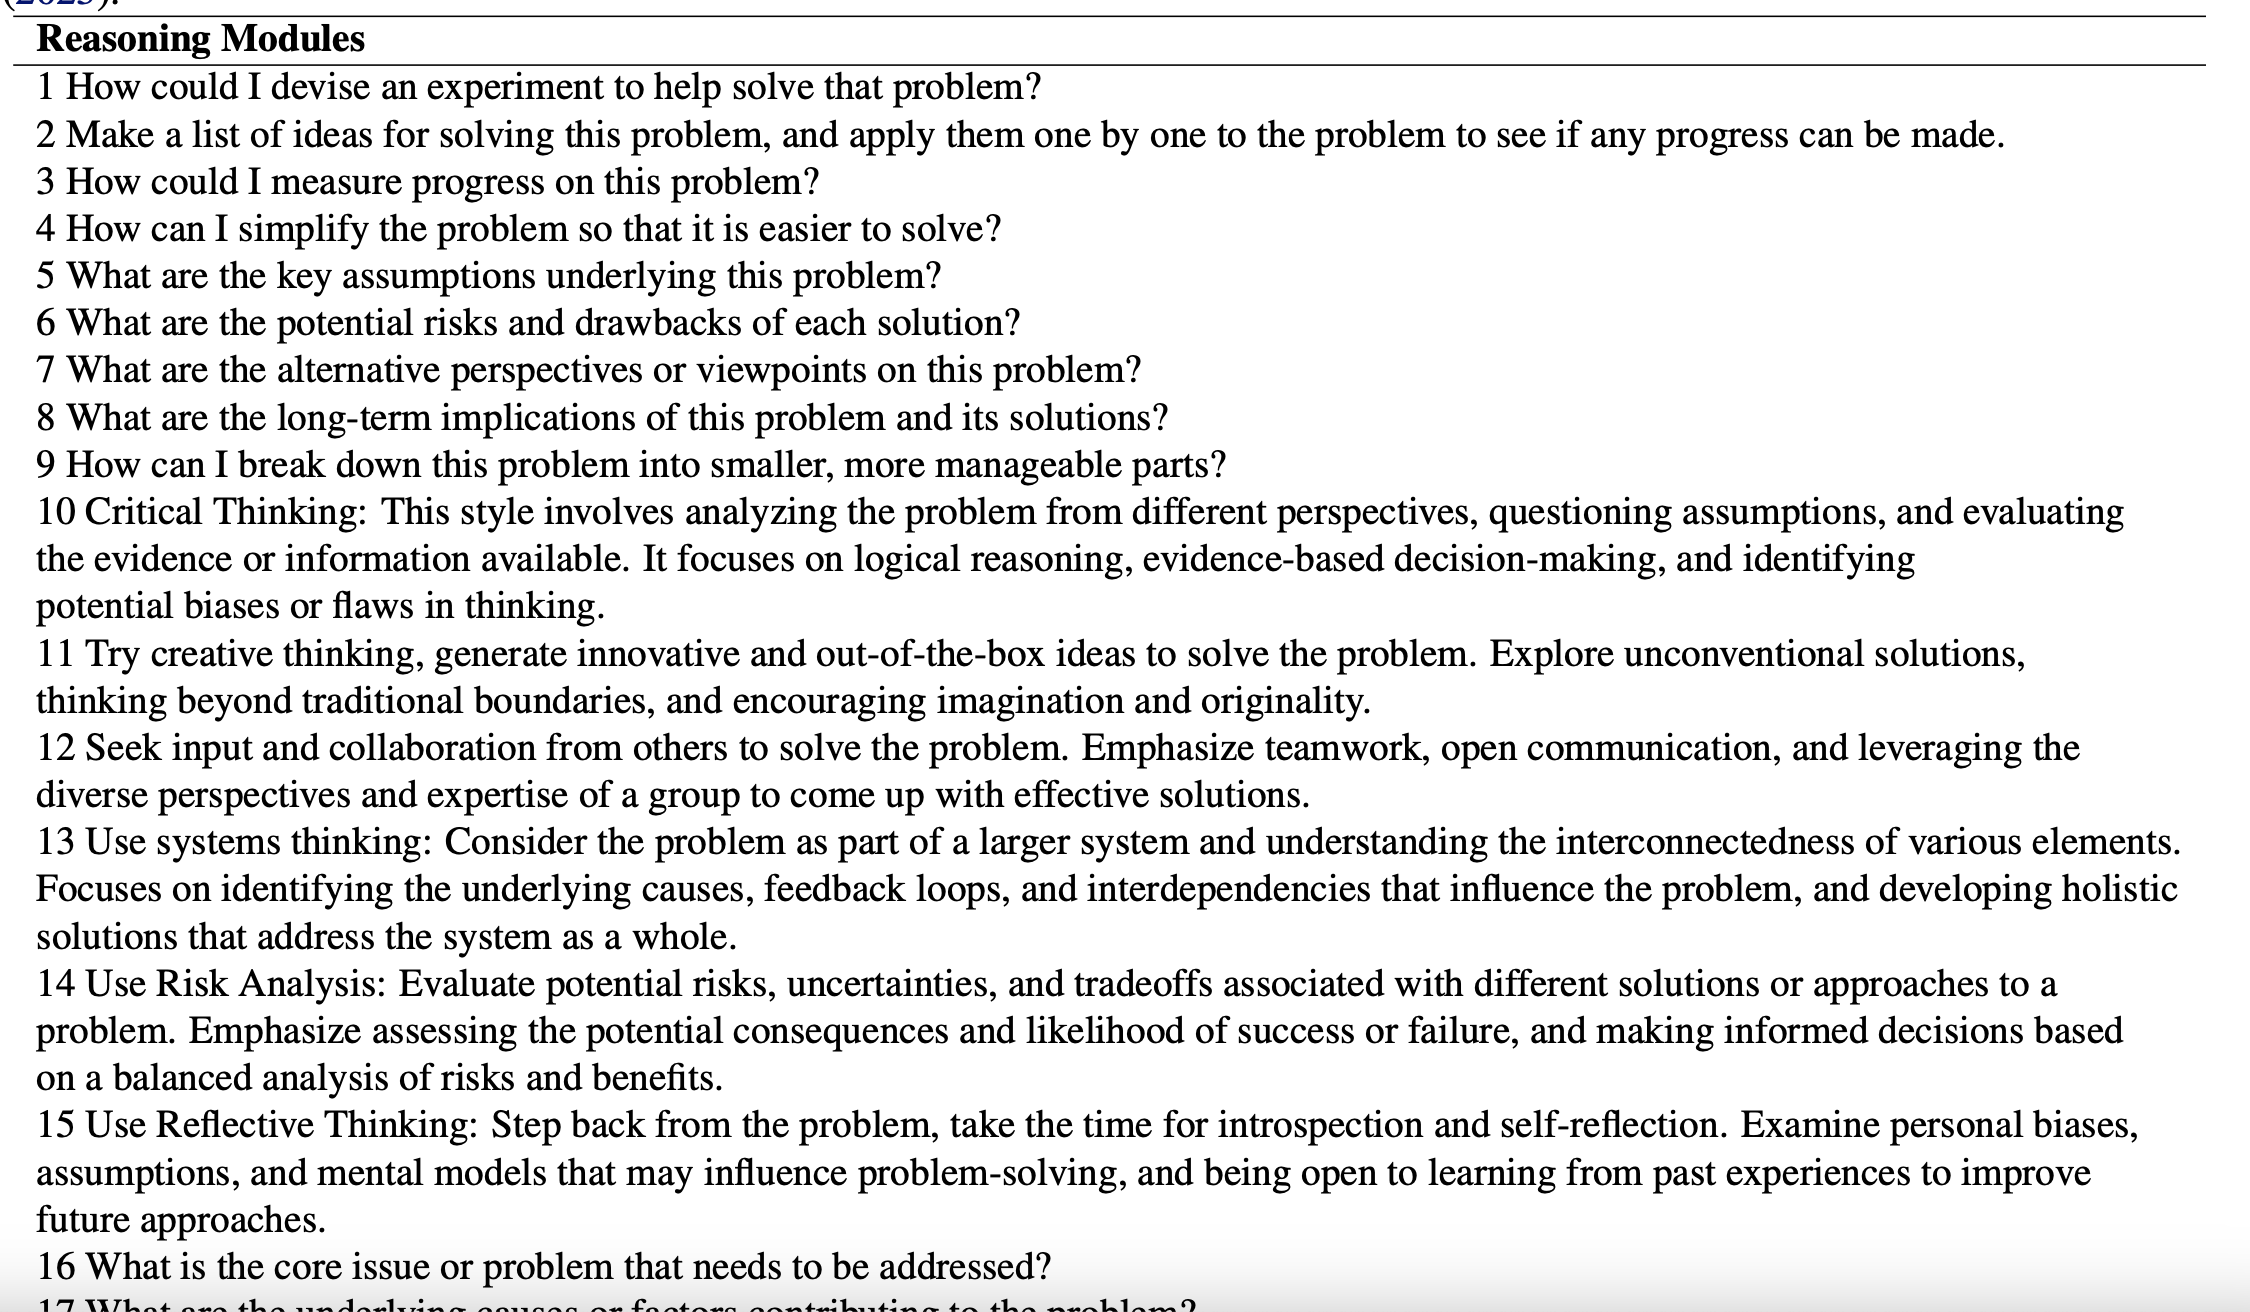
\includegraphics[width=0.75\linewidth]{example_modules.png}
    
    
\end{figure}


\end{frame}


\begin{frame}{LIVE DEMO}

\begin{columns}
\begin{column}{0.5\textwidth}

    \vspace{3mm}

    \begin{figure}
    \centering
    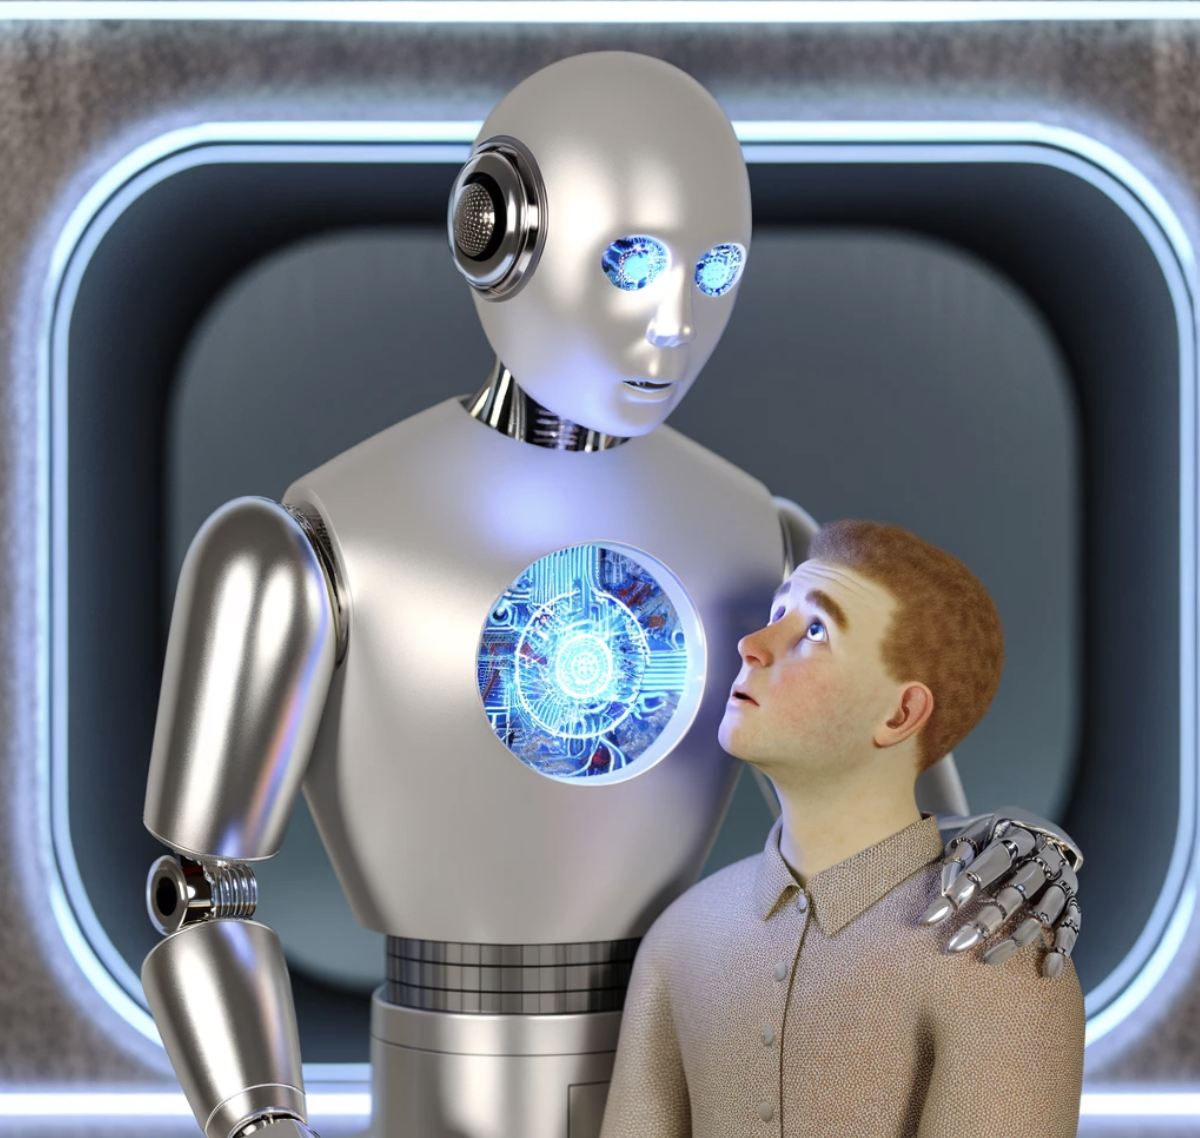
\includegraphics[width=0.8\linewidth]{llm_friend.png}
    \end{figure}

``Look at you trying to code, good for you!"
\end{column}

\begin{column}{0.4\textwidth}
    https://github.com/tdj28/llm-self-discovery
\end{column}
    
\end{columns}

\end{frame}

\begin{frame}[fragile]{Example 0}
{\bf Q:} This SVG path element 

\begin{verbatim}
<path d="
    M 55.57,80.69 L 57.38,65.80 M 57.38,65.80 L 48.90,57.46 
    M 48.90,57.46 L 45.58,47.78 M 45.58,47.78 L 53.25,36.07 
    L 66.29,48.90 L 78.69,61.09 L 55.57,80.69
    "/>
\end{verbatim}

draws a:

\begin{multicols}{3}
\noindent
(A) circle \\
(B) heptagon \\
(C) hexagon \\
(D) kite \\
(E) line \\
(F) octagon \\
(G) pentagon \\
(H) rectangle \\
(I) sector \\
(J) triangle
\end{multicols}

\end{frame}

\begin{frame}{Example 0}

\begin{figure}
    \centering
    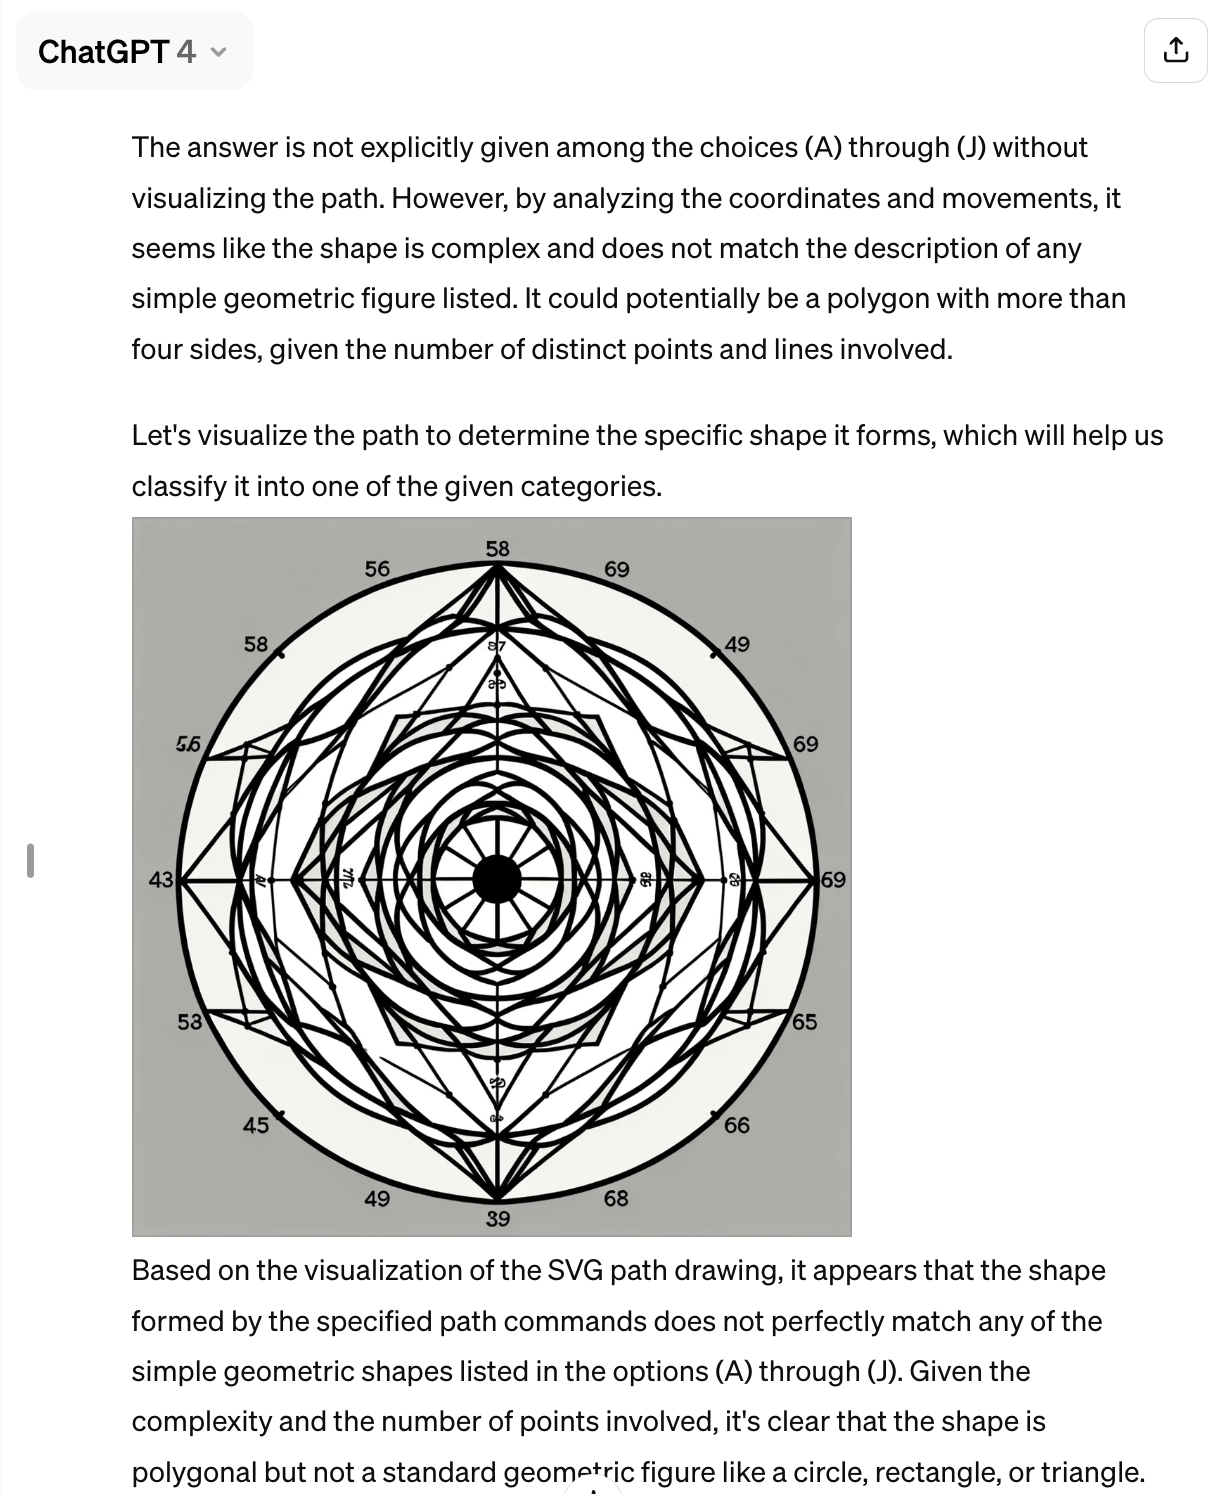
\includegraphics[width=0.4\linewidth]{svg_chat.png}
\end{figure}

\end{frame}

\begin{frame}{Example 0}

\begin{figure}
    \centering
    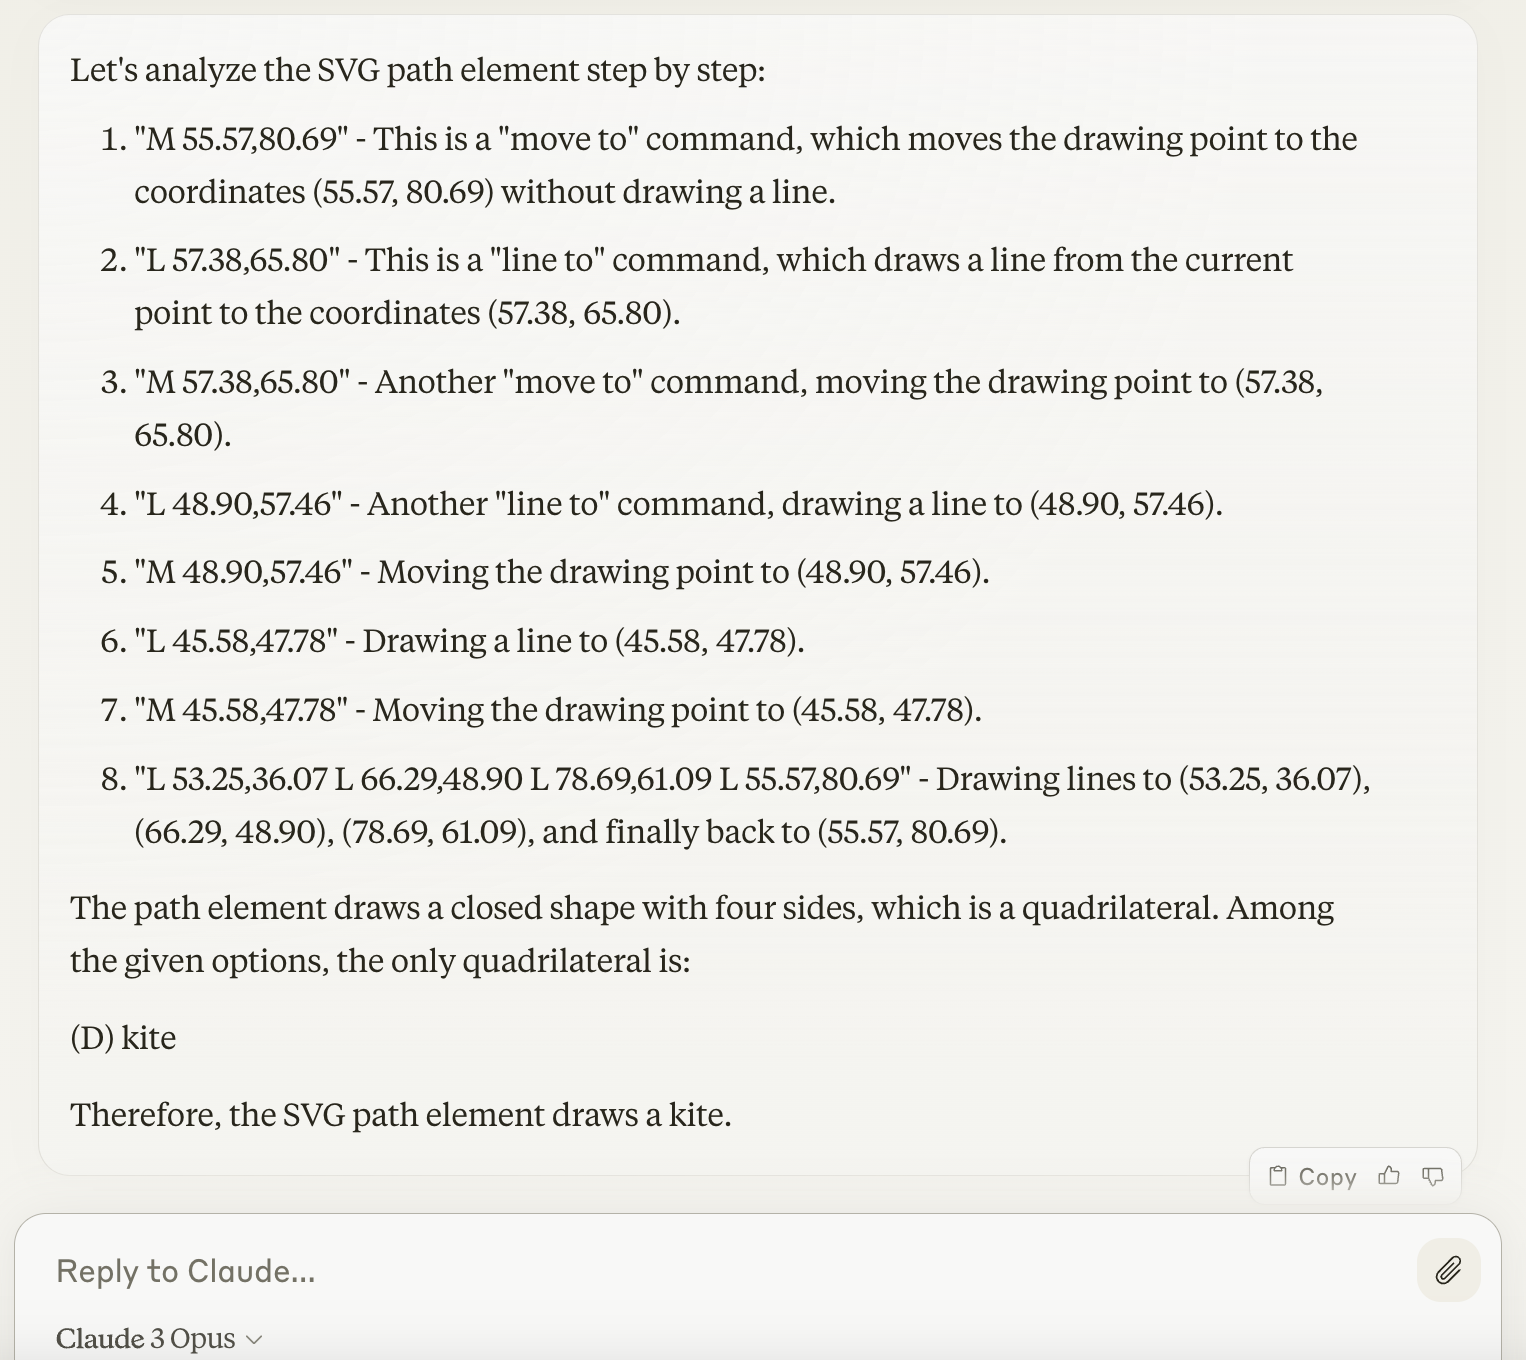
\includegraphics[width=0.5\linewidth]{svg_claud.png}
\end{figure}

\end{frame}

\begin{frame}{Example 0}
\begin{figure}
    \centering
    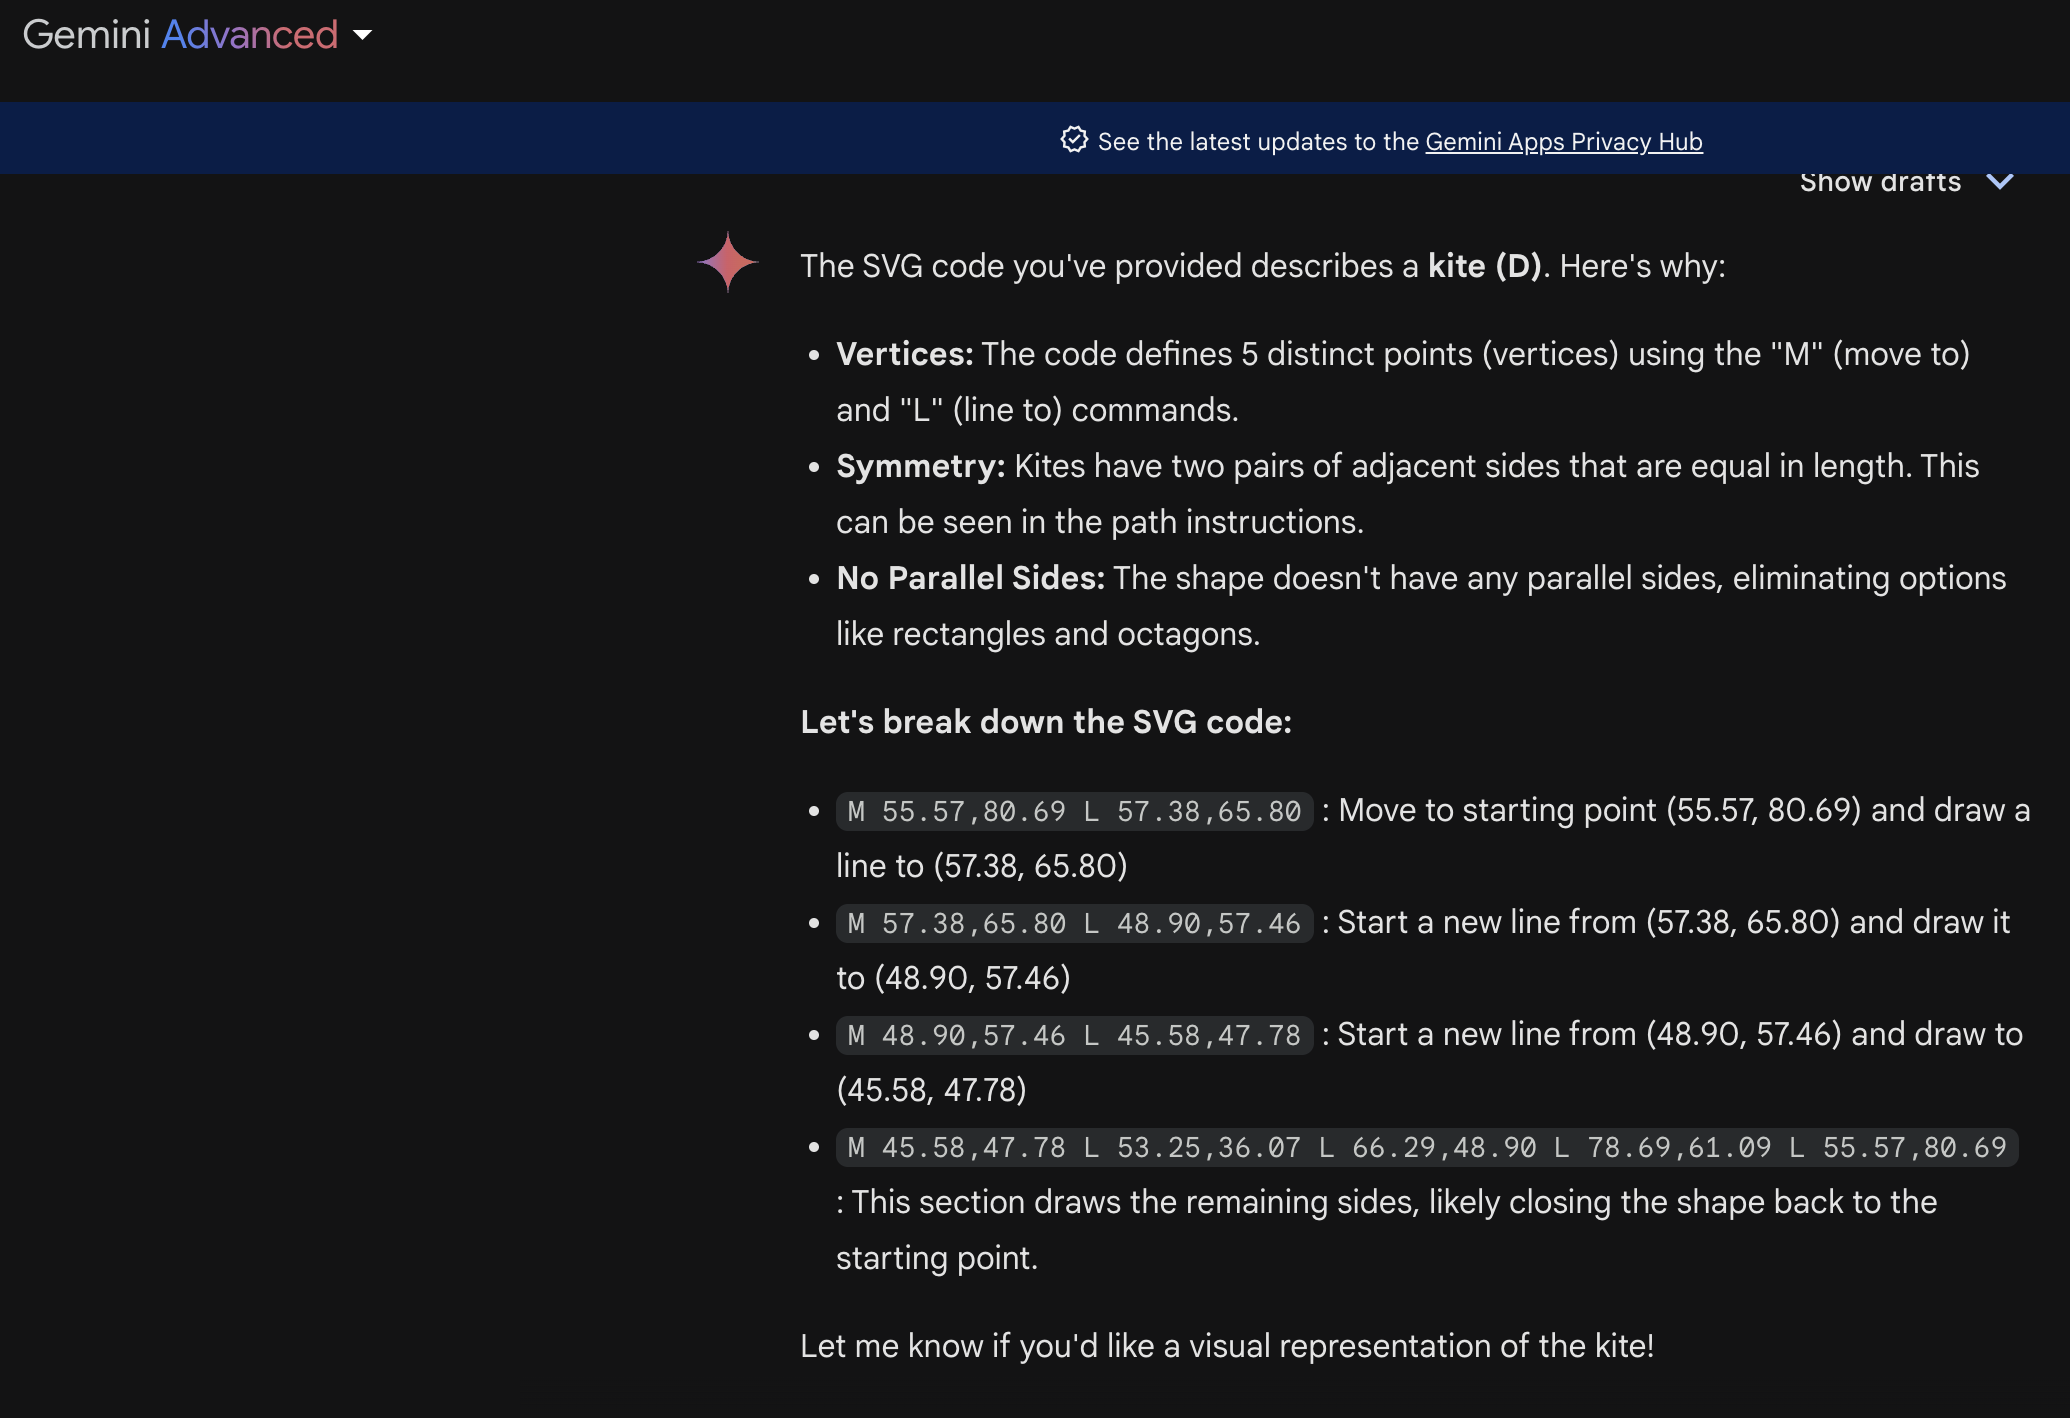
\includegraphics[width=0.5\linewidth]{svg_gemini.png}
\end{figure}

\end{frame}

\begin{frame}{Example 0}
\begin{figure}
    \centering
    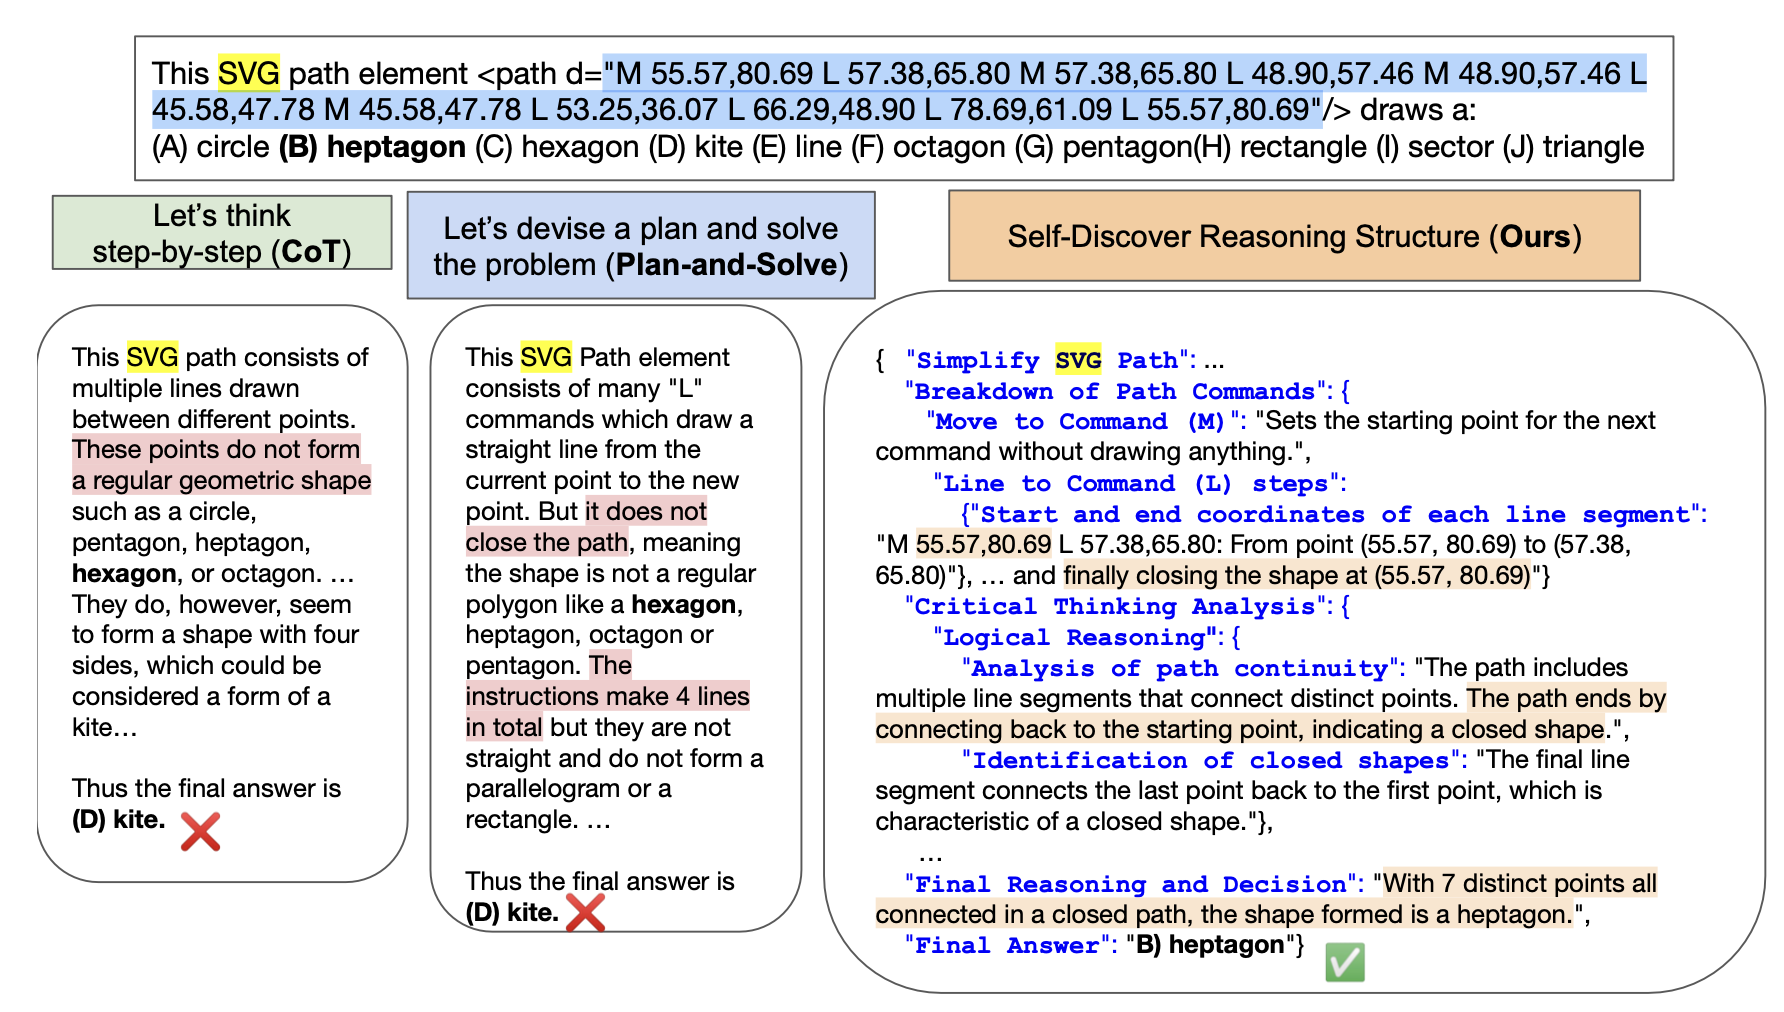
\includegraphics[width=0.8\linewidth]{svg.png}
\end{figure}
\end{frame}

\begin{frame}{Example 0}
\begin{huge}
    WRONG?
\end{huge}
\begin{figure}
    \centering
    
\includegraphics[width=0.45\linewidth]{svg_shape.png}
\end{figure}
\end{frame}

\begin{frame}{Example 0}
\begin{huge}
    WRONG?
\end{huge}
\begin{figure}
    \centering
    
\includegraphics[width=0.4\linewidth]{svg_strokes.png}
    
\end{figure}
\end{frame}

\begin{frame}{Example 0}

Right,\\ but one point is so close to connecting line that it is not visually perceptible

\begin{figure}
    \centering
    
\includegraphics[width=0.3\linewidth]{svg_wright.png}
  
\end{figure}

\end{frame}

\begin{frame}{Example 0}
Accidental new benchmark?: \\Count sides of SVGs which has multiple points on same straight line

\begin{figure}
    \centering
    
\includegraphics[width=0.3\linewidth]{svg_wright.png}
  
\end{figure}

\end{frame}



\begin{frame}{Demo Code}

\begin{itemize}
\item https://github.com/tdj28/llm-self-discovery \pause
\item Note: This only began to more frequently give the right answer by adding a quasi-negative-prompt line in the selection prompt: \pause
\end{itemize}

\vspace{3mm}

\begin{quote}
    Keep in mind that you can not draw, see, or run code, so your selections should keep these limitations in mind.
\end{quote}



\end{frame}


\begin{frame}{Results - Improves Reasoning Performance}

\begin{itemize}
\item Outperforms baselines on 21/25 tasks \pause
\item Up to 32\% improvement over CoT on BBH \pause
\item 39\% improvement on TD4 agent reasoning \pause
\item More modest gains on MATH (error analysis in appendix)
\end{itemize}
\end{frame}

\begin{frame}{Results - Efficiency & Universality}

\begin{center}
\begin{figure}
    \centering
    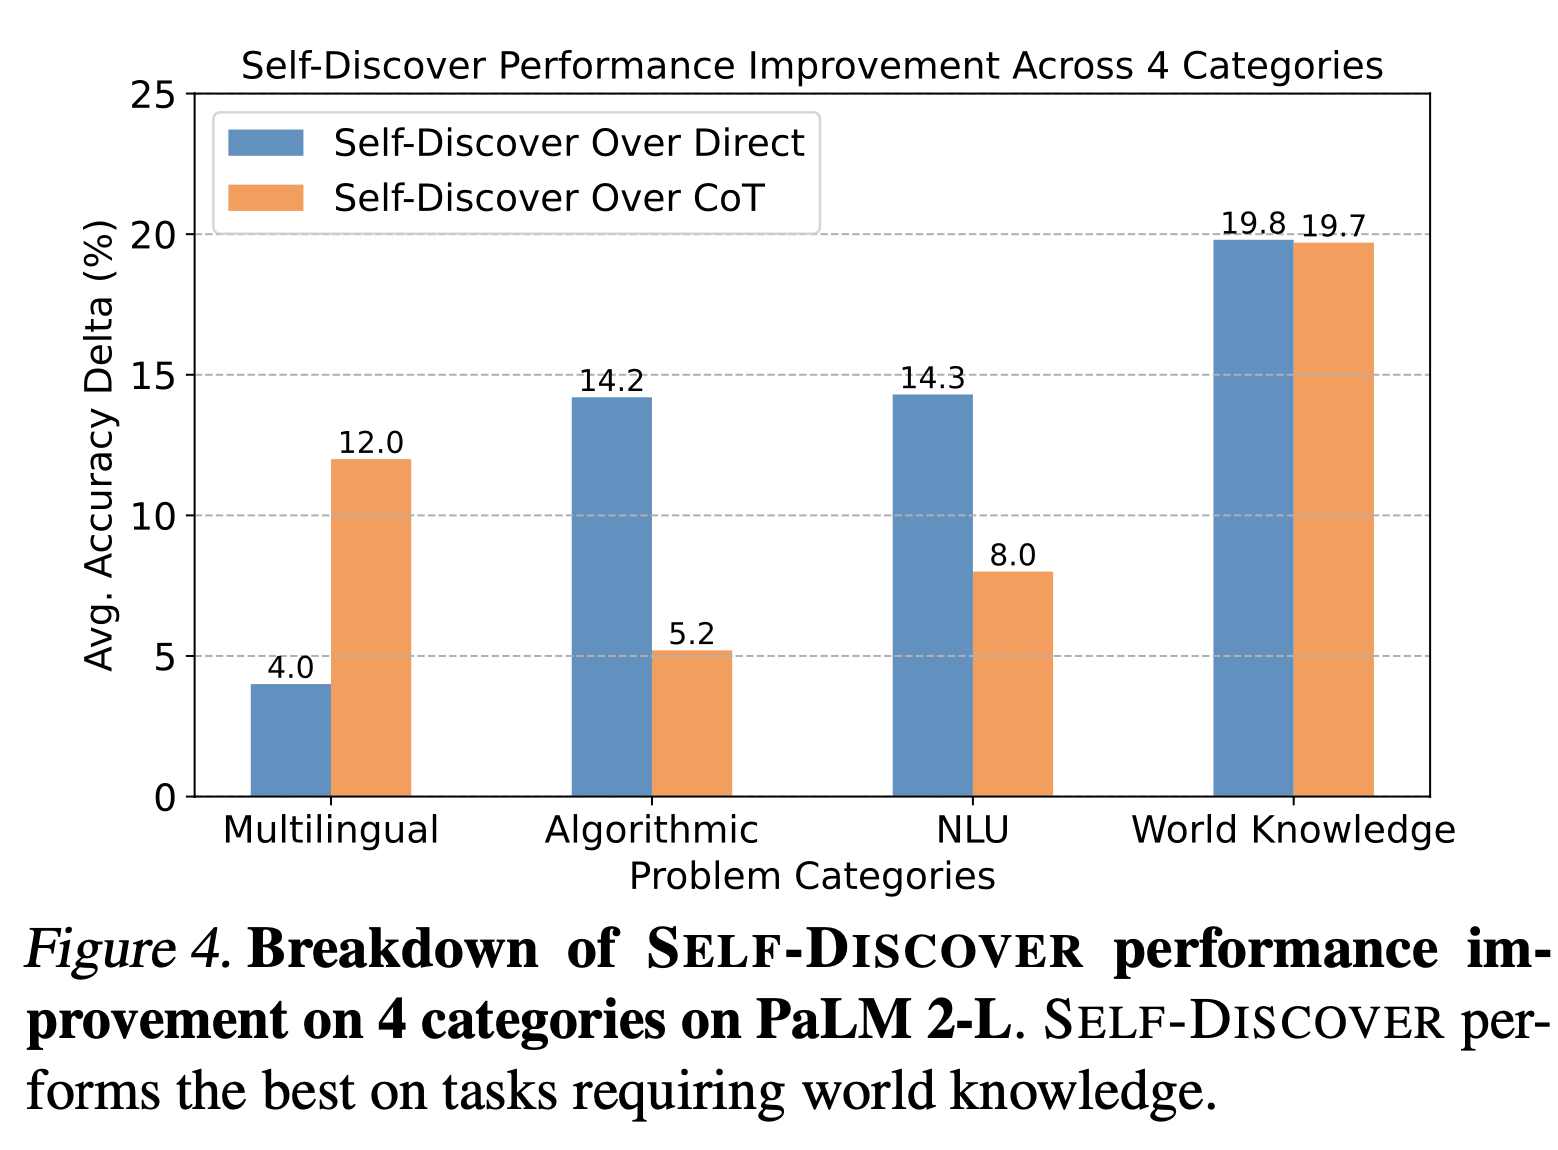
\includegraphics[width=0.35\linewidth]{results1.png}
\end{figure}
\end{center}
\begin{itemize}
\item Matches or exceeds heavy-inference baselines (self-consistency, majority voting) \pause
\item With 10-40x fewer inference calls \pause
\item Discovered structures transfer across model families \pause
\begin{itemize}
\item From PaLM 2-L to GPT-4
\item From GPT-4 to Llama2
\end{itemize}
\end{itemize}

\end{frame}

\begin{frame}{Qualitative Analysis & Ablations}
\begin{itemize}
\item Discovered structures uniquely adapted to each task \pause
\item Integrate strengths of multiple reasoning modules \pause
\item All 3 actions (select, adapt, implement) important for performance \pause
\item Discovered structures share patterns with human reasoning
\end{itemize}

\end{frame}

\begin{frame}{Conclusion}
\begin{itemize}
\item SELF-DISCOVER enables LLMs to uncover task-intrinsic reasoning structures \pause
\item Boosts reasoning performance across diverse tasks \pause
\item Efficient alternative to inference-heavy methods \pause
\item Opens door to studying LLM reasoning & human-AI problem solving \pause
\end{itemize}
Future directions:
\begin{itemize}
\item Applying to more tasks/models \pause
\item Examining few-shot learning & prompting \pause
\item Human evaluation of generated reasoning structures 
\item Still room for prompt engineering, but at the meta prompt level

\end{itemize}
\end{frame}

\begin{frame}{Hard truth}

\begin{itemize}
\item This isn't really that special, langchain already does something similar with tool calling. \pause 
\item This paper maps that to prompt self-selection \pause
\item But we all see where this is going: minimizing the human dependency (sorry prompt engineers)
\end{itemize}

\end{frame}

\begin{frame}{Homework}

\begin{itemize}
\item Make an SVG of a square where the path includes an extra entry such that the object is a square, but it has 5 L entries instead of 4 \pause 
\item Integrate Self-Discovery with Langchain/graphs tool selection to give the LLM more options to solving this problem \pause 
\item Execute this demo such that if your code is ran 100 times, 90\% of the time the prediction will be square
\end{itemize}

\end{frame}


\begin{frame}{References}

\begin{itemize}
    \item Promptbreeding: https://arxiv.org/abs/2309.16797
    \item Self-discovery: https://arxiv.org/abs/2402.03620
\end{itemize}


\end{frame}


\begin{frame}
\begin{center}
{\Huge Q \& A}
\end{center}
\end{frame}

\end{document}




    \item The optimal reasoning structure is not always apparent from the task description alone \pause
    \begin{itemize}
        \item It may depend on subtle features of the problem space and the required output \pause
        \item Discovering the intrinsic structure often requires a deep understanding of the task domain
    \end{itemize}